\documentclass[12pt,a4paper]{article}
\usepackage[margin=1in]{geometry}
\usepackage[moduleName=VRC6]{KautenjaDSP}
% import a debugging package to show the margin boxes
% \usepackage{showframe}
% set the graphics path to the img directory
\graphicspath{{img/}}

% algorithm2e stuff
% \SetKwInOut{Objects}{$\CKmatrix{O}$}
% \SetKwInOut{Weights}{$\CKvector{w}$}

\begin{document}
\titlePage{VRC6-Logo}{VRC6-Module}{KautenjaDSP}

% -------------------
% MARK: Overview
% -------------------

\section{Overview}

VRC6 is an emulation of the Konami VRC6 sound chip from the Nintendo Entertainment System (NES) for VCV Rack. The VRC6 chip contains two pulse wave generators, and a quantized saw wave generator.

VRC6 provides the key features of the VRC6 chip, namely,
\begin{itemize}
  \item \textbf{Dual pulse wave generator:} Dual 8-bit pulse waves with eight duty cycles: $6.25\%$, $12.5\%$, $18.75\%$, $25\%$, $31.25\%$, $37.5\%$, $43.75\%$, and $50\%$;
  \item \textbf{Quantized saw wave generator:} Generate NES style saw wave with variable quantization;
  \item \textbf{Amplitude modulation:} Manual and CV control over the individual voice levels
\end{itemize}

% -------------------
% MARK: Panel Layout
% -------------------

\clearpage
\section{Panel Layout}

\begin{figure}[!htp]
\centering
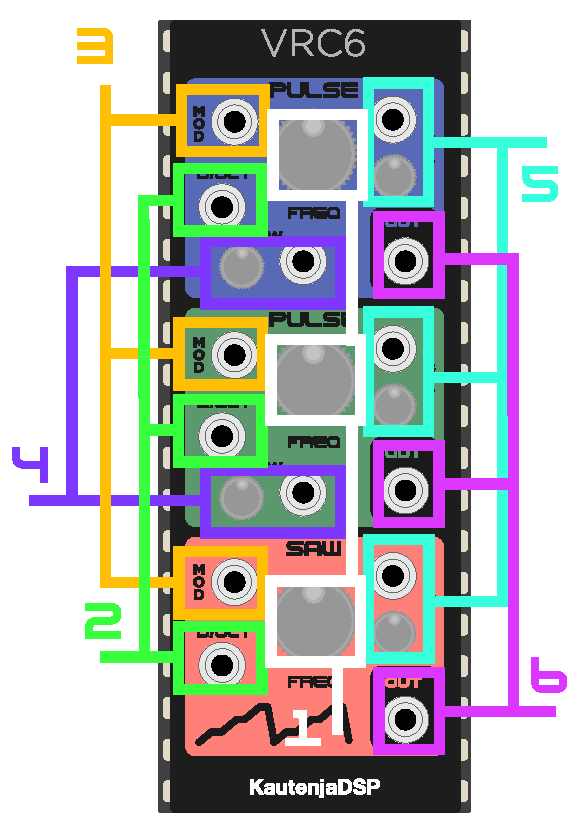
\includegraphics{VRC6-Manual}
\end{figure}

\begin{enumerate}
  \item Coarse frequency control for the pulse1, pulse2, and saw waveform generators.
  \item $V$/Octave inputs for pulse1, pulse2, and saw waveform generators.
  \item linear CV frequency modulation for pulse1, pulse2, and saw generators.
  \item Pulse width selector. Chooses between eight duty cycles: $6.25\%$, $12.5\%$, $18.75\%$, $25\%$, $31.25\%$, $37.5\%$, $43.75\%$, and $50\%$. CV control is discretized into $2V$ windows per stage.
  \item Coarse amplitude control over the oscillator using the 4-bit amplifier. When no input is connected, the slider controls the level from $0\%$ to $100\%$. When an input is connected, the slider acts as an attenuator.
  \item Channel outputs, ${\approx}10V_{pp}$.
\end{enumerate}

% -------------------
% MARK: References
% -------------------

\clearpage
\renewcommand\refname{References \& Acknowledgments}
\nocite{*}
\bibliographystyle{apalike}
\bibliography{references}

\end{document}
